% Trabajo sobre el modelo del hiperboloide
% Autores:
% * Margarita Gómez
% * Eva María González
% * David Melero
% * Mario Román
%
% Usando la plantilla de beamer de Pablo Baeyens.
% Autor: Pablo Baeyens (@pbaeyens)
% Email: pbaeyens31+github@gmail.com
% Licencia: CC BY-SA 3.0

%% Paquetes y configuración %

% Beamer
\PassOptionsToPackage{unicode}{hyperref}  % Evita errores con caracteres no ASCII
\PassOptionsToPackage{naturalnames}{hyperref} % tex.stackexchange.com/questions/10555
\documentclass[compress]{beamer}

% Idioma
\usepackage[spanish]{babel} % Traducciones
\usepackage[utf8]{inputenc} % Uso de caracteres UTF-8
\usepackage{lmodern}        % Fuentes de tamaño arbitrario
\usepackage[T1]{fontenc}    % Permite copiar y evita errores
\uselanguage{Spanish}       % Traducciones beamer
\languagepath{Spanish}      % (tex.stackexchange.com/questions/168208)

% Matemáticas
\usepackage{amsfonts}
\usepackage{amsmath}
\usepackage{amssymb}

% Colores
\definecolor{backg}{HTML}{F2F2F2}    % Fondo
\definecolor{title}{HTML}{bdc3d1}    % Títulos
\definecolor{comments}{HTML}{BDBDBD} % Comentarios
\definecolor{keywords}{HTML}{08388c} % Palabras clave
\definecolor{strings}{HTML}{FA5858}  % Strings
\definecolor{links}{HTML}{2C2C95}    % Enlaces
\definecolor{bars}{HTML}{045FB4}     % Barras (gráfico)

% Código
\usepackage{listings}
\lstset{
language=[LaTeX]TeX,
basicstyle=\footnotesize,
morekeywords={href,uselanguage,languagepath,column},
otherkeywords={pause,usetheme,usecolortheme,useinnertheme,titlepage,tableofcontents,subtitle},
breaklines=true,
backgroundcolor=\color{backg},
keywordstyle=\color{keywords},
commentstyle=\color{comments},
stringstyle=\color{strings},
tabsize=2,
% Acentos, ñ, ¿, ¡ (tex.stackexchange.com/questions/24528)
extendedchars=true,
literate={á}{{\'a}}1 {é}{{\'e}}1 {í}{{\'i}}1 {ó}{{\'o}}1
         {ú}{{\'u}}1 {ñ}{{\~n}}1 {¡}{{\textexclamdown}}1
         {¿}{{?`}}1
}

% Gráficos
\usepackage{pgfplots}
\pgfplotsset{width=7cm,compat=1.8} % Opciones para gráficos

% Emoticonos
\usepackage{wasysym}

% tikz
\usepackage{tikz}
\usetikzlibrary{mindmap,trees,shadows}
\tikzset{ % Genera overlays
    invisible/.style={opacity=0},
    visible on/.style={alt={#1{}{invisible}}},
    alt/.code args={<#1>#2#3}{\alt<#1>{\pgfkeysalso{#2}}{\pgfkeysalso{#3}}},
}

%% Comandos %%
\newcommand{\ejemplo}[1]{\lstinputlisting{./examples/#1}} % Mostrar código de ejemplos
\newcommand{\muestra}[1]{\input{./examples/#1}}           % Mostrar ejemplos
\newcommand{\seccion}[1]{\input{./sections/#1}}           % Incluir secciones
\newcommand{\espacio}{\vspace*{\baselineskip}}            % Añade espacios
\newcommand{\beamer}{\texttt{beamer} }                    % Estilo único para beamer
\newcommand{\enlace}[3]{\href{#1}{\textbf{#2}} - {\small #3}}  % Estílo único para refs
\newcommand{\comando}[1]{{\color{black}\textbackslash}{\color{keywords}#1}}

%% Temas %%
% Tema y tema de color
  \usetheme{Dresden}
  \usecolortheme{dolphin}
  \useinnertheme{circles}
  \setbeamercovered{transparent}
% Colores bloques
  \setbeamercolor{block title}{bg=title,fg=links}
  \setbeamercolor{block body}{bg=backg,fg=black}
  \setbeamercolor{block title alerted}{fg=red!70!black,bg=title!92!red}
  \setbeamercolor{block body alerted}{fg=black,bg=backg}
  \setbeamercolor{block title example}{fg=green!70!black,bg=title!92!green}
  \setbeamercolor{block body example}{fg=black,bg=backg}
% Enlaces (tex.stackexchange.com/questions/13423)
\hypersetup{colorlinks,linkcolor=,urlcolor=links}
% Quita enlaces de navegación (stackoverflow.com/questions/3017030)
\setbeamertemplate{navigation symbols}{}
% Quita barra inferior (stackoverflow.com/questions/1435837)
\setbeamertemplate{footline}{}
% Evita warnings boxes
\hfuzz=20pt
\vfuzz=20pt
% Evita wranings itemize
\renewcommand\textbullet{\ensuremath{\bullet}}

%% Título y otros %%
\title{Modelo del hiperboloide}                                               % Título
\subtitle{Y otros modelos para la geometría hiperbólica}                                  % Subtítulo
\author[UGR]{ %
Eva Mª González \and Margarita Gómez  \\ David Melero \and Mario Román \texorpdfstring{\\
\href{}{}}{}} % Autor y e-mail
\date{Taller de geometría y topología}                                                            % Fecha


%% Presentación %%
\begin{document}

\begin{frame}
\titlepage
\end{frame}

\begin{frame}{Índice}
  \hypertarget{index}{}
  \tableofcontents
\end{frame}

\section{Disco de Poincaré}
\begin{frame}{Modelo para un sistema}
  Un \textbf{modelo} para un sistema de postulados se define sustituyendo objetos específicos
  por los términos indefinidos del sistema.

  \pause
  \begin{exampleblock}{Ejemplo: geometría euclídea}
    Un modelo de la geometría euclídea es el que asigna a cada punto un par de reales $(a,b)$
    y a cada recta el conjunto de puntos que satisfacen una ecuación lineal $as+bt+u = 0$ para
    algunos reales tales que al menos uno de ellos no sea $0$.
  \end{exampleblock}
\end{frame}

\begin{frame}{Disco de Poincaré}
  El modelo de Poincaré se define tomando

  \begin{itemize}
  \item \textbf{puntos} como puntos contenidos en un círculo unidad. Es decir,
    como pares de reales $(a,b)$ cumpliendo $a^2+b^2 < 1$.
    \pause
  \item \textbf{líneas} como los puntos interiores al círculo unidad de otra circunferencia
    que lo corta perpendicularmente.
    \pause
  \item los \textbf{ángulos} entre dos rectas hiperbólicas como el ángulo que
    proporcionan las tangentes a las rectas en el punto de corte.
  \end{itemize}
\end{frame}

\begin{frame}{Teselación con hexágonos rectos}
  Podemos teselar un plano hiperbólico con hexágonos con todos sus ángulos rectos.
  Nótese que todos ellos son \textit{congruentes} (!).
  
  \begin{centering}
    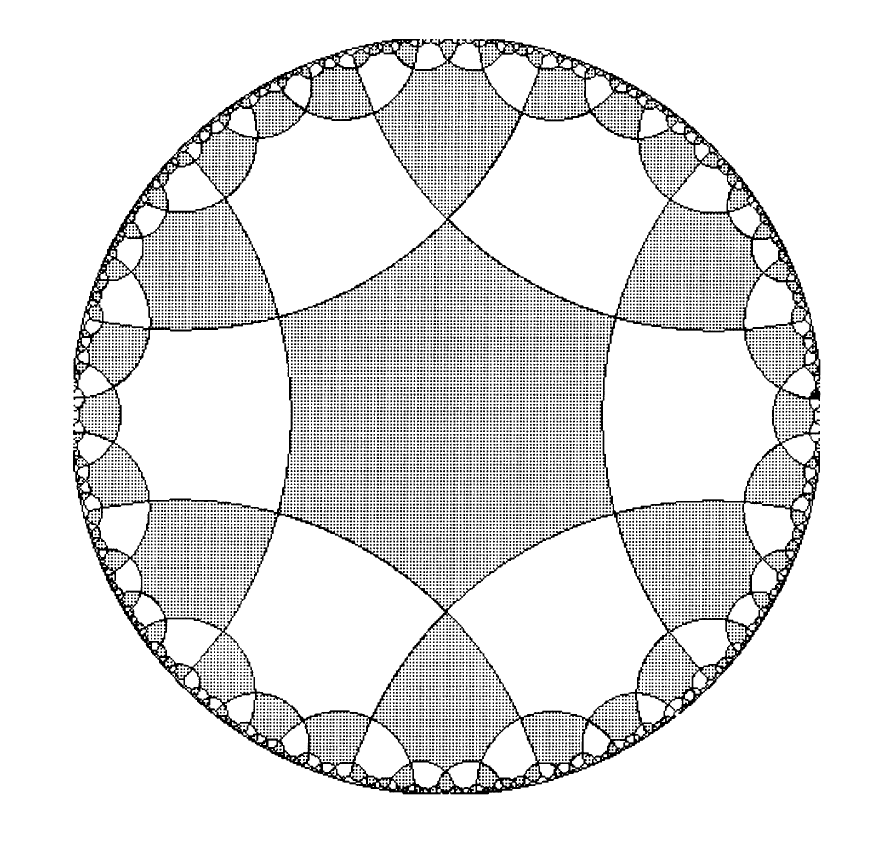
\includegraphics[width=0.5\textwidth]{teselahexagonos.png}
  \end{centering}
\end{frame}

\begin{frame}{Relación con el modelo del hiperboloide}
  Los puntos del disco de Poincaré están en correspondencia con los puntos del modelo
  del hiperboloide. La correspondencia se obtiene proyectando desde el punto $(0,0,-1)$.

  \begin{itemize}
  \item Dado un punto $(x,y,z)$ en el hiperboloide (cumpliendo por tanto $z^2-x^2-y^2 = 1$),
    su proyección será
    \[\frac{1}{1+z}(x,y).\]
    \pause
  \item Dado un punto $(0,a,b)$ en el disco (cumpliendo por tanto $a^2+b^2 < 1$), su
    proyección será
    \[\frac{1}{1-a^2-b^2}\left(1+a^2+b^2,2a,2b\right).\]
  \end{itemize}
\end{frame}

\end{document}
